%%%%%%%%%%%%%%%%%%%%%%%%%%%%%%%%%%%%%%%%%%%%%%%%%
% FINAL REPORT
%%%%%%%%%%%%%%%%%%%%%%%%%%%%%%%%%%%%%%%%%%%%%%%%%

\documentclass[a4paper,10.5pt,twoside]{article}
\hyphenpenalty=8000
\textwidth=125mm
\textheight=200mm

\usepackage{fancyhdr}
\pagestyle{fancy}
\fancyhead{}
\fancyfoot{}
\raggedbottom

\usepackage{xurl}
\usepackage{graphicx}
\usepackage{alltt}
\usepackage{subcaption}
\usepackage{amsmath}
\usepackage[hidelinks]{hyperref}
\urlstyle{same}
\usepackage[T1]{fontenc}
\usepackage[utf8]{inputenc}
\usepackage{lmodern}
\usepackage{csquotes}
\usepackage{comment}
\usepackage{float}
\usepackage{xcolor}
\usepackage[a4paper, top=3cm, bottom=2cm, left=3cm, right=3cm]{geometry}
\usepackage[english]{babel}
\usepackage{booktabs}
\usepackage{longtable}
\usepackage{array}
\usepackage{enumitem}

\pagenumbering{arabic}
\setcounter{page}{1}

\hypersetup{
    colorlinks=true,
    linkcolor=blue,
    citecolor=blue,
    urlcolor=blue
}

\begin{document}

\fancyhead[LE]{\thepage\ \ \ MBD Final Report}
\fancyhead[RO]{African Multimodal Adaptation\ \ \ \thepage}

\begin{center}
{\Large \textbf{African-Context Adaptation for Multimodal Image--Text Misinformation Detection}}\\[12pt]
{\normalsize
Ishimwe Karekezi Guy Gael\\
Lynne Chepkwony\\
Emile Lucky Muhigira
}
\end{center}

\begin{abstract}
Multimodal misinformation often appears as an authentic image paired with misleading text that reframes the event, place, or actors shown. This form of misinformation is difficult to catch with text-only or image-only systems because the deception lies in the relationship between the two modalities. In this project we study whether lightweight multimodal consistency features derived from a pretrained contrastive model can support misinformation detection in African media contexts, and whether adapting a benchmark-trained model with African-context data improves performance without harming the original benchmark. We combine CLIP-based image--text features with a logistic regression classifier, beginning with a Fakeddit baseline and extending the evaluation to a manually curated African-context dataset of 178 local image--text examples. We compare four views of the same pipeline: baseline performance on Fakeddit, direct transfer from Fakeddit to Africa before adaptation, adapted performance on an unseen African holdout, and the adapted model's performance on the original Fakeddit test set.

The final system yields strong in-domain performance on Fakeddit and shows that African-context adaptation improves target-domain behavior in the metrics most relevant to misinformation screening, especially misinformation recall and misinformation F1. At the same time, the adapted model remains strong on Fakeddit and even improves on the benchmark in the current configuration. These results suggest that benchmark-trained multimodal misinformation systems can benefit from targeted African adaptation, and that this adaptation can be achieved with a lightweight, explainable pipeline suitable for practical deployment in resource-constrained settings.
\end{abstract}

\section{Introduction}
Misinformation on digital platforms is increasingly multimodal. Rather than fabricating an entire image, many misleading posts recycle a real image and attach new text that changes the implied location, date, event, or political meaning. The resulting image--text pair may be highly persuasive because each component appears individually plausible, while the misinformation emerges from the mismatch between them. This makes multimodal misinformation detection an important but challenging problem.

Much recent work in multimodal misinformation detection has relied on large supervised architectures, late fusion systems, or external knowledge sources \cite{khattar2020spotfake,li2024kamp}. These methods can be effective, but they are often difficult to reproduce and costly to deploy. In low-resource environments, practical systems benefit from approaches that are smaller, easier to analyze, and compatible with modest compute budgets. Pretrained contrastive models such as CLIP offer an attractive alternative because they provide rich image and text representations that can be reused without expensive end-to-end training \cite{radford2021clip}.

Our project began from a simple question: can semantic consistency between an image and its accompanying text act as a reliable signal for multimodal misinformation risk? As the project evolved, a second question became central: even if such a system works on benchmark datasets, how well does it perform on African-context examples, and can targeted adaptation improve that performance? This second question matters because African digital content is frequently underrepresented in mainstream benchmarks, while the social and political stakes of misinformation remain high.

The final contribution of this work is therefore twofold. First, we build a practical misinformation detector using CLIP-derived image--text consistency features and a logistic regression classifier. Second, we move beyond benchmark-only evaluation by creating and testing on an African-context dataset, then adapting the model with African training examples. This lets us ask not only whether the model can transfer to African contexts, but whether adaptation can improve target-domain performance while preserving the benchmark capabilities that made the original model attractive.

\paragraph{Main contributions.}
This final report makes the following contributions:
\begin{itemize}[leftmargin=1.5em]
    \item A lightweight multimodal misinformation detection pipeline using CLIP-based consistency features and logistic regression.
    \item An African-context evaluation dataset of 178 locally stored image--text examples for robustness testing and adaptation experiments.
    \item An empirical comparison of four setups: Fakeddit baseline, Fakeddit-to-Africa transfer, African adaptation on an unseen African holdout, and benchmark preservation after adaptation.
    \item A deployable Streamlit application that uses the adapted model and exposes human-readable explanations of the prediction.
\end{itemize}

\section{Related Work}
Multimodal misinformation detection has developed rapidly over the last several years. Early systems such as SpotFake combined text and visual features with supervised fusion architectures to identify fake news \cite{khattar2020spotfake}. Later work explored richer multimodal pretraining and knowledge-aware representations \cite{li2024kamp}. In parallel, benchmark datasets such as Fakeddit \cite{nakamura2019fakeddit}, VisualNews \cite{liu2021visualnews}, MM-COVID \cite{li2020mmcovid}, and NewsCLIPpings \cite{luo2021newsclippings} helped standardize experimental evaluation.

A recurring lesson from this literature is that multimodal misinformation is often not about falsified pixels, but about contextual mismatch. NewsCLIPpings, for example, focuses on out-of-context media reuse, where an image is real but paired with misleading text \cite{luo2021newsclippings}. This framing is especially relevant to our work because the African-context dataset we assembled contains many such cases: protest photos reused for the wrong country, public-order images linked to the wrong election, or archived scenes described as current events.

At the same time, many widely used multimodal benchmarks are dominated by data from Western or global platforms. That raises the question of domain shift. If a model is optimized on a benchmark like Fakeddit, there is no guarantee it will behave similarly on African-context data. This is not simply a geographic issue; it includes differences in reporting style, protest imagery, languages, source quality, local institutions, and the kinds of misleading narratives that circulate online.

This concern connects our work with a broader literature on representation gaps and dataset imbalance in African AI research. Although that literature often focuses on language resources and hate speech rather than misinformation directly, the underlying issue is similar: models built from globally dominant datasets do not necessarily capture African communicative contexts well \cite{muhammad2025afrihate}. A closely related point is made in recent work on multimodal misinformation in a South African social media setting, which highlights the importance of evaluating methods on regionally grounded data rather than assuming benchmark transfer will be sufficient \cite{dejager2023southafrica}.

Our project differs from much prior work in two ways. First, we deliberately use a lightweight classifier over pretrained multimodal features rather than a heavy end-to-end neural system. Second, we focus the final evaluation on adaptation: not simply whether the benchmark model works on Africa, but whether adding African training examples improves target-domain performance while preserving the original benchmark strength.

\section{Problem Definition}
We formulate the task as binary classification over image--text pairs:
\begin{itemize}[leftmargin=1.5em]
    \item \textbf{misinformation}: the text misrepresents, reframes, or falsely contextualizes the image;
    \item \textbf{likely consistent}: the text appears semantically compatible with the image.
\end{itemize}

The detector does not attempt to establish factual truth in the full fact-checking sense. Instead, it estimates misinformation \emph{risk} from semantic consistency between the visual and textual modalities. This is an important distinction: a mismatch between image and text can be a useful signal of misinformation, but not every true claim is visually obvious, and not every visually plausible claim is true. We therefore position the model as a screening tool rather than an automated fact-checker.

The main research questions are:
\begin{enumerate}[leftmargin=1.5em]
    \item Can pretrained multimodal consistency features support a strong lightweight baseline for image--text misinformation detection?
    \item How robust is a Fakeddit-trained model when evaluated directly on African-context examples?
    \item Does adaptation with African training data improve African performance while preserving strength on Fakeddit?
\end{enumerate}

\section{Data Sources and Dataset Construction}
\subsection{Benchmark data: Fakeddit}
The main benchmark dataset used in this project is Fakeddit \cite{nakamura2019fakeddit}, a large-scale multimodal dataset derived from Reddit posts. Each example includes text, image metadata, and misinformation-oriented labels. From the original multimodal table of 564,000 rows, we filtered to examples with non-null image and text content, sampled a manageable subset, recovered locally available images, and built a CLIP-ready modeling table.

The resulting benchmark modeling subset contains 9,979 usable image--text examples. This subset is large enough to support stable training and model comparison while remaining practical for the course project's compute budget.

\begin{figure}[H]
\centering
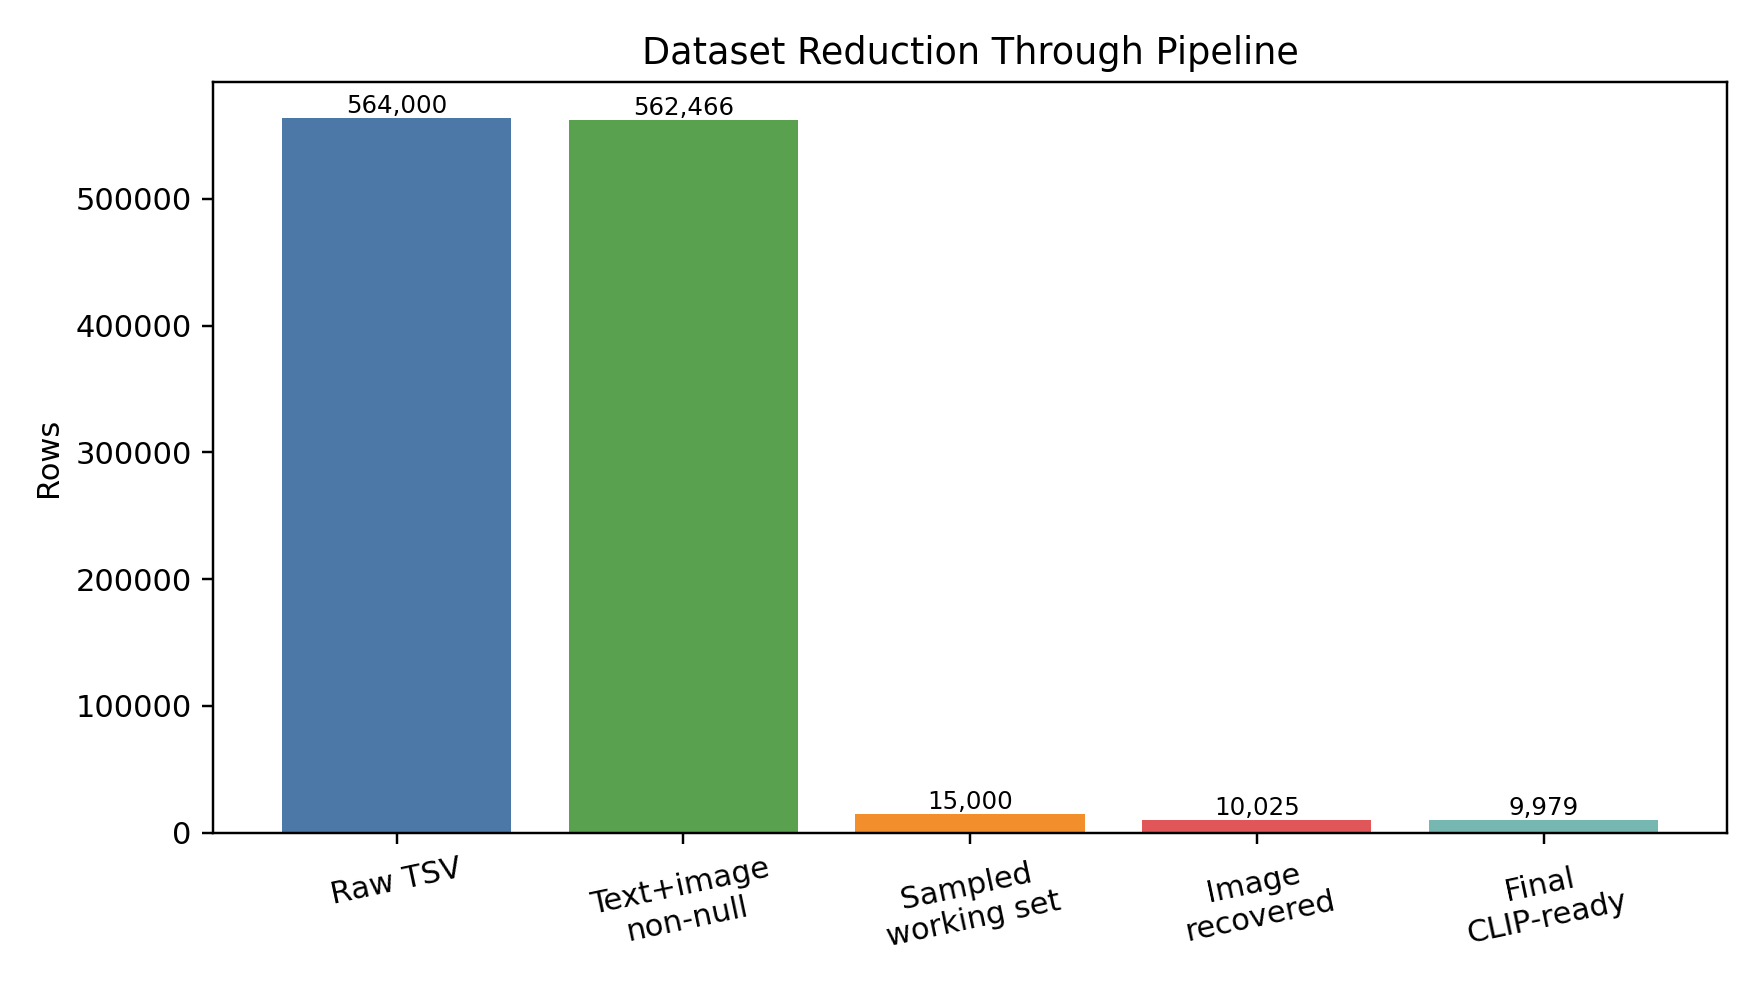
\includegraphics[width=0.95\linewidth]{figures/data_pipeline_counts.png}
\caption{Reduction from the raw Fakeddit multimodal table to the final CLIP-ready modeling subset.}
\label{fig:data_pipeline}
\end{figure}

\begin{figure}[H]
\centering
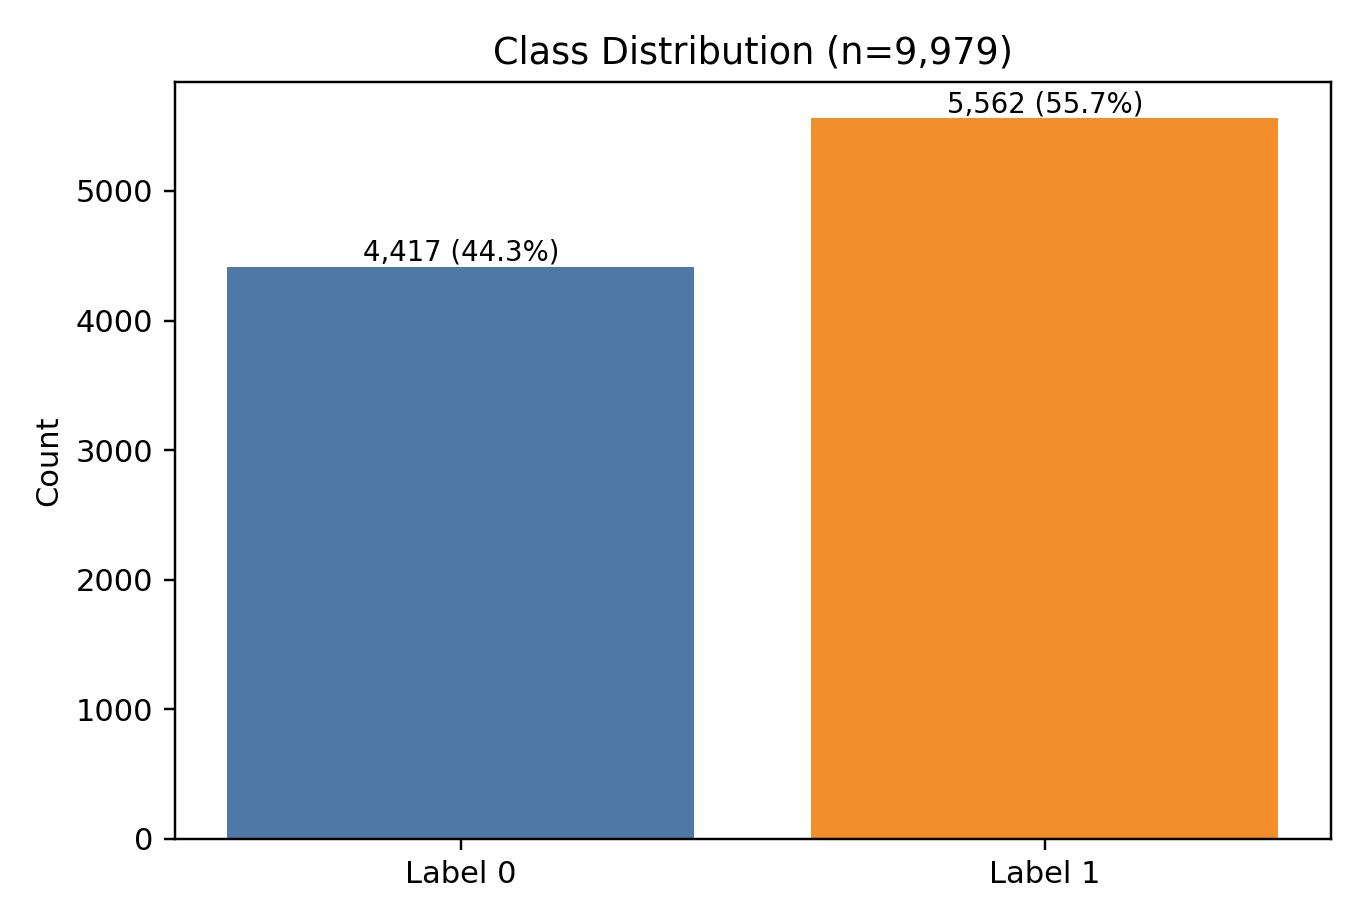
\includegraphics[width=0.72\linewidth]{figures/class_distribution.png}
\caption{Class balance in the Fakeddit modeling subset used for the baseline classifier.}
\label{fig:class_distribution}
\end{figure}

\subsection{African-context dataset}
To evaluate contextual robustness, we built a separate African-context dataset of locally stored image--text examples. This dataset grew beyond the original proposal's small manual test set and now contains 178 examples with one row per image. The data combines:
\begin{itemize}[leftmargin=1.5em]
    \item manually assembled local image--text examples curated by the team;
    \item additional sourced examples linked to African fact-checking and news contexts;
    \item both \texttt{misinformation} and \texttt{likely\_consistent} labels.
\end{itemize}

Every example is stored locally in the project image folder and referenced through a relative path. The dataset is therefore stable for reproducible evaluation and application demos.

The current dataset statistics are:
\begin{itemize}[leftmargin=1.5em]
    \item Total examples: 178
    \item Unique image files referenced: 178
    \item \texttt{misinformation}: 81
    \item \texttt{likely\_consistent}: 97
\end{itemize}

The topic distribution is intentionally diverse, with strong representation for public-order scenes, community events, sports, health, education, water access, public expression, and livelihood-related content. This diversity matters because African misinformation frequently appears in political, civic, and humanitarian settings where contextual framing is central.

\begin{table}[H]
\centering
\caption{African-context dataset summary.}
\label{tab:african_summary}
\begin{tabular}{lr}
\toprule
Statistic & Value \\
\midrule
Total rows & 178 \\
Unique image paths & 178 \\
Misinformation rows & 81 \\
Likely consistent rows & 97 \\
African train split & 142 \\
African holdout split & 36 \\
Holdout label balance & 18 misinformation / 18 likely consistent \\
\bottomrule
\end{tabular}
\end{table}

\subsection{Data quality and annotation}
The African dataset was curated with practical safeguards. We favored public-scene images over sensitive close-up portraits, avoided unnecessary defamation against identifiable private individuals, and emphasized visible scene grounding when writing captions. Team labeling was discussed collaboratively, and difficult cases were reviewed before inclusion. While some examples are synthetic in the sense that the misleading text was deliberately composed, they were designed to mimic common real-world reframing patterns such as wrong location, wrong event, or misleading crisis framing.

\section{Methodology}
\subsection{Feature construction with CLIP}
We use the pretrained CLIP ViT-B/32 model \cite{radford2021clip} to encode each image and its paired text. Given normalized image embedding $v$ and text embedding $t$, we construct a feature vector that combines:
\begin{enumerate}[leftmargin=1.5em]
    \item the cosine similarity $\cos(v,t)$,
    \item the absolute embedding difference $|v - t|$,
    \item the concatenated image and text embeddings $[v;t]$.
\end{enumerate}

This produces a fixed feature representation that captures both global alignment and fine-grained modality differences. The same feature construction is used for Fakeddit and the African dataset, which keeps the adaptation comparison fair.

\subsection{Classifier}
On top of the CLIP-derived features, we train a logistic regression classifier. This choice was motivated by three considerations:
\begin{itemize}[leftmargin=1.5em]
    \item interpretability relative to deeper architectures;
    \item computational efficiency for repeated experiments;
    \item strong empirical performance on the benchmark subset.
\end{itemize}

The midterm experiments compared several candidate models and found that the logistic regression baseline achieved the strongest ROC-AUC while remaining stable under cross-validation. The relevant benchmark figures are retained in the final report because they justify the choice of the lightweight classifier.

\begin{figure}[H]
\centering
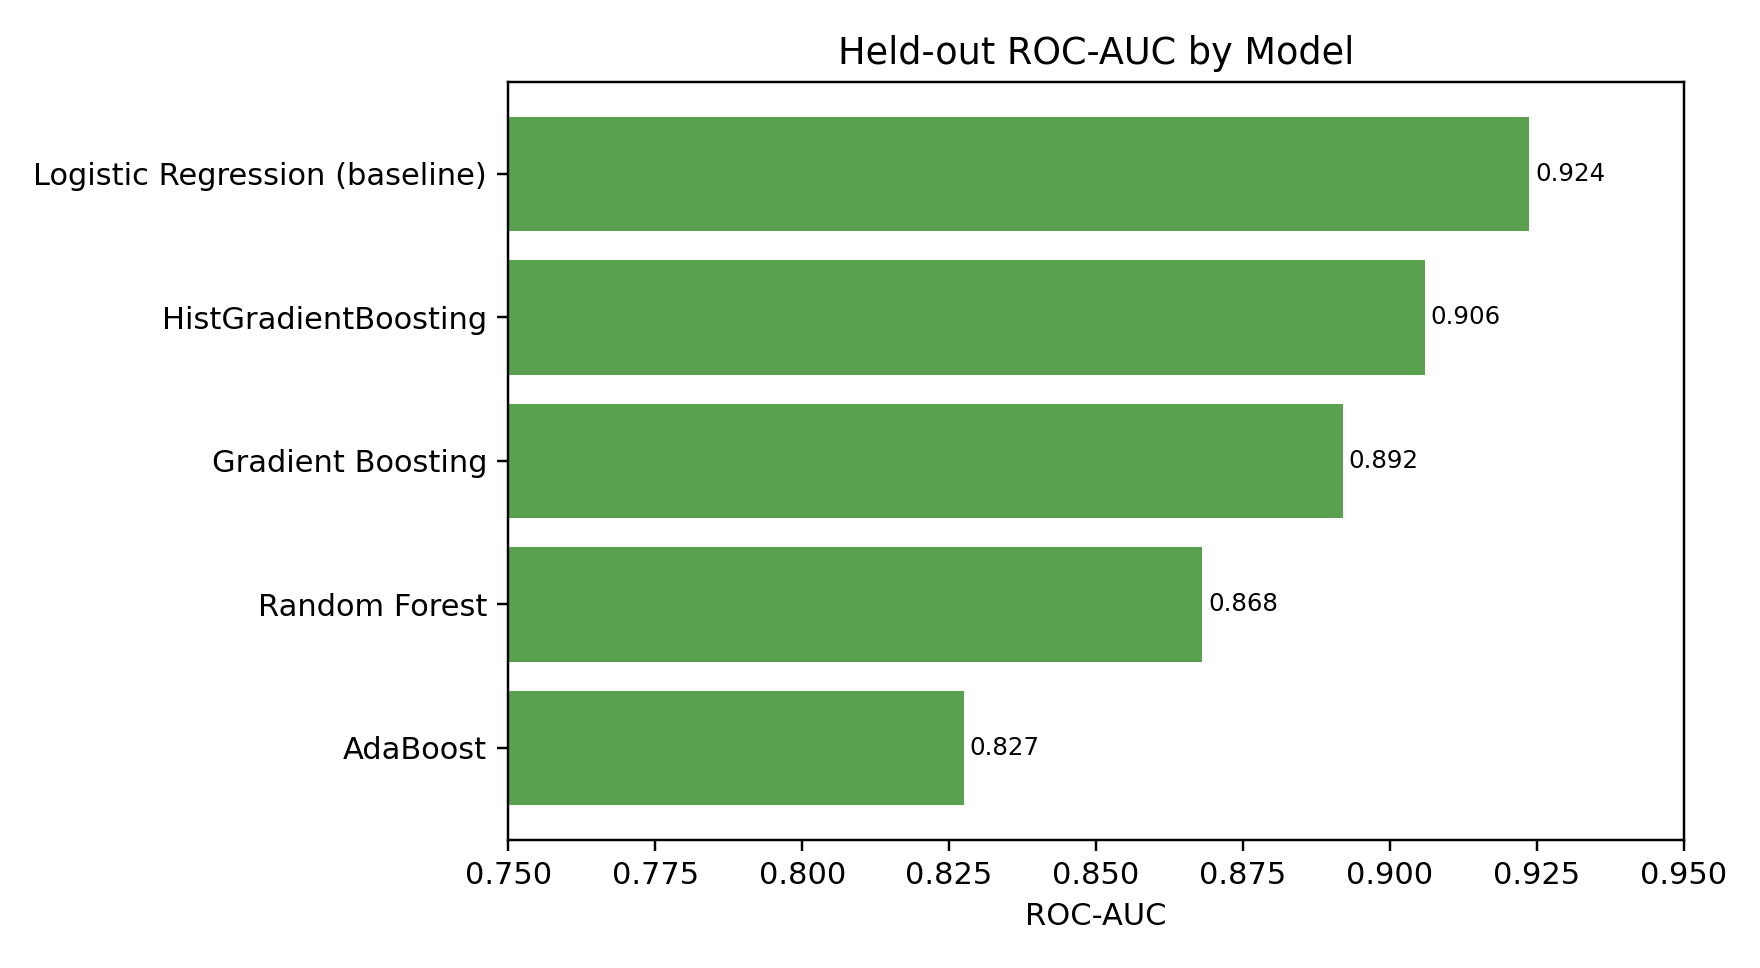
\includegraphics[width=0.95\linewidth]{figures/model_comparison_rocauc.png}
\caption{Held-out ROC-AUC comparison among candidate models in the benchmark stage. Logistic regression provided the strongest lightweight baseline.}
\label{fig:model_compare}
\end{figure}

\begin{figure}[H]
\centering
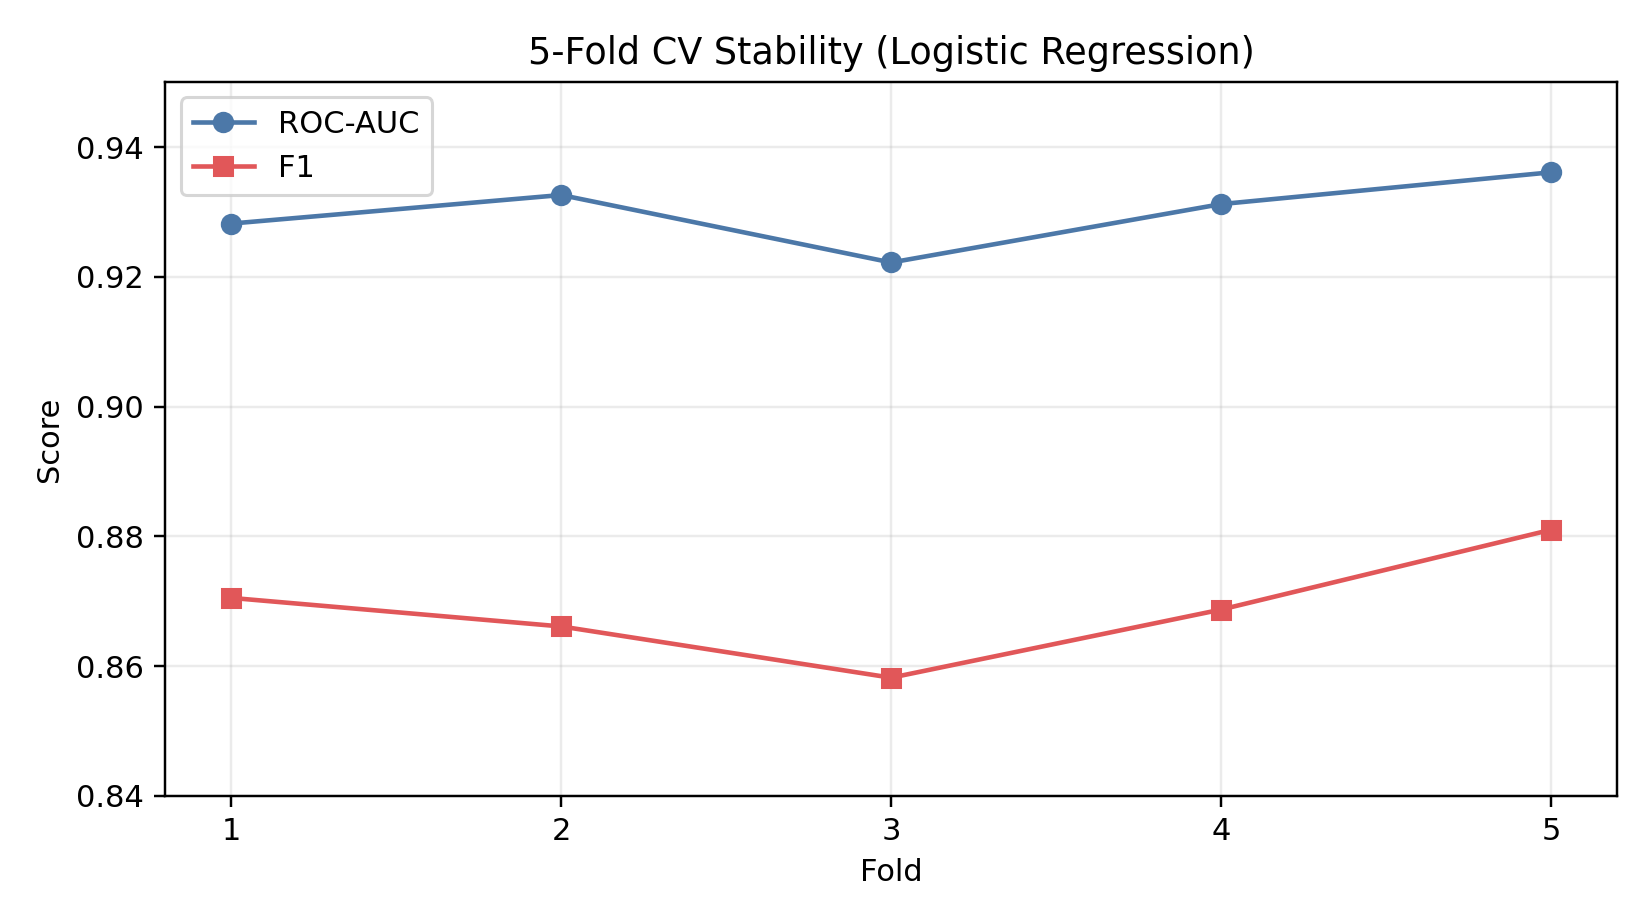
\includegraphics[width=0.9\linewidth]{figures/cv_stability.png}
\caption{Cross-validation stability of the logistic regression baseline on the Fakeddit subset.}
\label{fig:cv_stability}
\end{figure}

\subsection{Adaptation protocol}
The adaptation process has four key stages:
\begin{enumerate}[leftmargin=1.5em]
    \item Train the original baseline on the Fakeddit train split.
    \item Evaluate that baseline on Fakeddit and then directly on the African dataset before adaptation.
    \item Split the African dataset into an African-train portion and an unseen African holdout portion.
    \item Train an adapted logistic regression model on the combined set of Fakeddit training examples and African-train examples, then evaluate on the African holdout and on the original Fakeddit test set.
\end{enumerate}

To reduce the risk of overfitting, the African holdout was never used while selecting the adapted model hyperparameters. Instead, tuning was done using grouped validation on the available training-side data only. The best observed setting for the adapted model used a balanced class weight and $C=10.0$.

\section{Experimental Setup}
\subsection{Setup A: Original model on Fakeddit}
This setup measures in-domain benchmark performance using the original Fakeddit-trained model on the held-out Fakeddit test set.

\subsection{Setup B: Original model on Africa before adaptation}
This setup applies the same original model directly to the African dataset, without any African training examples. It serves as the pre-adaptation reference point.

\subsection{Setup C: Adapted model on African holdout}
For the main adaptation result, we split the African dataset into 142 African-train examples and 36 African holdout examples. The adapted model is trained on Fakeddit plus African-train, and then evaluated on the unseen African holdout.

\subsection{Setup D: Adapted model on Fakeddit}
Finally, we evaluate the adapted model on the original Fakeddit test set. This preservation check asks whether African adaptation damages, preserves, or improves the source-domain benchmark.

\section{Results}
\subsection{Benchmark baseline}
The original model achieved strong in-domain performance on Fakeddit:
\begin{itemize}[leftmargin=1.5em]
    \item Accuracy: 0.8473
    \item Macro F1: 0.8457
    \item Misinformation precision: 0.8179
    \item Misinformation recall: 0.8424
    \item Misinformation F1: 0.8300
\end{itemize}

These metrics confirm that the CLIP-plus-logistic-regression baseline is competitive on the benchmark subset used in the project.

\subsection{African performance before adaptation}
Direct evaluation on the African dataset produced a weaker result:
\begin{itemize}[leftmargin=1.5em]
    \item Accuracy: 0.6685
    \item Macro F1: 0.6336
    \item Misinformation precision: 0.7619
    \item Misinformation recall: 0.3951
    \item Misinformation F1: 0.5203
\end{itemize}

The confusion matrix for this setup showed that the model was much better at identifying likely consistent examples than misinformation examples. In particular, African misinformation recall dropped substantially relative to the benchmark behavior, which is strong evidence of domain mismatch.

\subsection{African performance after adaptation}
After adaptation with African training examples, the African holdout performance improved in the metrics most relevant to misinformation detection:
\begin{itemize}[leftmargin=1.5em]
    \item Accuracy: 0.6667
    \item Macro F1: 0.6667
    \item Misinformation precision: 0.6667
    \item Misinformation recall: 0.6667
    \item Misinformation F1: 0.6667
\end{itemize}

Although overall accuracy remained similar to the pre-adaptation result, the adapted model achieved a much stronger balance across classes. Most importantly, misinformation recall increased from 0.3951 to 0.6667, and misinformation F1 increased from 0.5203 to 0.6667. For a misinformation screening tool, this improvement is more important than a small change in plain accuracy because missing misinformation carries a larger downstream risk.

\subsection{Preservation on Fakeddit after adaptation}
The adapted model also remained strong on the original benchmark:
\begin{itemize}[leftmargin=1.5em]
    \item Accuracy: 0.9078
    \item Macro F1: 0.9068
    \item Misinformation precision: 0.8854
    \item Misinformation recall: 0.9094
    \item Misinformation F1: 0.8972
\end{itemize}

In the current experiment, this is not merely preservation but improvement. The adapted model outperformed the original benchmark model on the held-out Fakeddit test set. This result strengthens the practical value of the adaptation approach: adding African-context data did not harm the original benchmark performance and may have improved general robustness.

\begin{table}[H]
\centering
\caption{Main experimental comparison across benchmark, transfer, and adaptation setups.}
\label{tab:main_results}
\begin{tabular}{p{4.0cm}p{3.2cm}ccccc}
\toprule
Comparison & Setup & Accuracy & Macro F1 & Misinfo Prec. & Misinfo Rec. & Misinfo F1 \\
\midrule
Original model on Fakeddit & Fakeddit $\rightarrow$ Fakeddit & 0.8473 & 0.8457 & 0.8179 & 0.8424 & 0.8300 \\
Original model on Africa before adaptation & Fakeddit $\rightarrow$ Africa & 0.6685 & 0.6336 & 0.7619 & 0.3951 & 0.5203 \\
Adapted model on Africa holdout & Fakeddit + Africa $\rightarrow$ Africa & 0.6667 & 0.6667 & 0.6667 & 0.6667 & 0.6667 \\
Adapted model on Fakeddit & Fakeddit + Africa $\rightarrow$ Fakeddit & 0.9078 & 0.9068 & 0.8854 & 0.9094 & 0.8972 \\
\bottomrule
\end{tabular}
\end{table}

\section{Discussion}
\subsection{What adaptation improved}
The clearest improvement from African adaptation appears in misinformation recall and misinformation F1 on the African holdout. This is important because the pre-adaptation model was overly conservative: it tended to classify African examples as likely consistent even when they were labeled as misinformation. Adaptation reduced that failure mode.

This improvement aligns with the intuition that African-context examples contain scene types, claims, and narrative patterns that are underrepresented in Fakeddit alone. By adding African training examples, the classifier becomes better calibrated for the target domain.

\subsection{Why accuracy is not the whole story}
The African accuracy changed only slightly, from 0.6685 before adaptation to 0.6667 after adaptation. At first glance, that can make the adaptation look less impressive than it really is. However, the class-sensitive metrics reveal the more meaningful story. Misinformation recall increased sharply, and macro F1 also improved. In a misinformation setting, this matters because a system that misses many misleading posts can be less useful than one that has slightly lower accuracy but catches more misinformation.

\subsection{Why the Fakeddit preservation result matters}
The final preservation check is not secondary. It answers a practical deployment concern: if we adapt the model with African data, do we damage the benchmark behavior that made the original system useful? In our current results, the answer is no. The adapted model remains strong on Fakeddit and even improves. This suggests that African adaptation does not merely specialize the model narrowly for a target domain; it may also improve the quality of the learned decision boundary more broadly.

\subsection{Implications for African digital content research}
The strongest interpretation of these results is not that we have solved African multimodal misinformation detection, but that benchmark-only training is not enough. African evaluation changed the story of the project. What began as a baseline misinformation detector became a study of domain adaptation for underrepresented media contexts. That shift is itself a contribution, because it highlights the importance of contextual evaluation and localized data in building practical misinformation tools.

\section{Tooling and Deployment}
A major project goal was not only analysis but also a functional tool. We therefore built a Streamlit-based application that:
\begin{itemize}[leftmargin=1.5em]
    \item accepts an uploaded image and associated text;
    \item computes the same CLIP-based consistency features used during training;
    \item returns a misinformation-risk prediction;
    \item provides a lightweight explanation, including feature-group contributions and word-level influence estimates.
\end{itemize}

The demo now prefers the adapted model by default once the notebook exports \texttt{adapted\_model.pkl} into the demo folder. This ensures that the application reflects the final adaptation-focused results rather than the earlier benchmark-only baseline.

The codebase and materials also include:
\begin{itemize}[leftmargin=1.5em]
    \item a GitHub repository containing the notebook, app, and data paths;
    \item local African image storage for reproducible evaluation;
    \item documentation for collection, labeling, and validation workflows.
\end{itemize}

\section{Ethical Considerations and Limitations}
This project raises several ethical issues. First, the model does not determine factual truth; it estimates semantic mismatch and misinformation risk. That means it can produce both false positives and false negatives. False positives may unfairly flag correct content, while false negatives may allow harmful misinformation to pass through.

Second, the African dataset is still limited in size and scope. Although it is much stronger than the small evaluation set originally envisioned in the proposal, it is not yet representative of the full diversity of African media environments. Topic balance is imperfect, and some examples remain manually curated or synthetic in their text framing.

Third, some misinformation examples involve politically sensitive or potentially harmful narratives. We attempted to reduce ethical risk by avoiding unnecessary defamation of private individuals and by preferring public-scene images where possible. Even so, any deployment of such a system should keep a human in the loop.

Fourth, the strong Fakeddit preservation result should be interpreted with care. It is encouraging, but it does not mean the adapted model is universally fair across all domains or languages. It means that, within the current project setup, African adaptation did not hurt the original benchmark and may have improved general robustness.

\section{Conclusion}
This final project demonstrates that a lightweight multimodal misinformation detector based on pretrained CLIP features and logistic regression can achieve strong benchmark performance and can be meaningfully improved for African-context use through targeted adaptation. The original Fakeddit-trained model performed well in-domain but was substantially weaker on African examples, especially for misinformation recall. After adaptation with African training examples, target-domain misinformation detection improved, while benchmark performance remained strong and even improved in the current experiments.

The project therefore contributes both a working tool and a research finding: African-context data matters, and adaptation can improve multimodal misinformation detection without necessarily sacrificing source-domain utility. For future work, the most important next steps are expanding the African dataset, improving metadata quality, introducing multilingual text coverage, and evaluating on additional African misinformation scenarios beyond the current manually curated collection.

\section*{Supplementary Materials}
The accompanying project materials include:
\begin{itemize}[leftmargin=1.5em]
    \item the GitHub repository with the notebook, Streamlit application, and saved models;
    \item the local African dataset CSV and image folder documentation;
    \item collection and annotation guidance used by the team;
    \item the midterm and proposal drafts that document the evolution of the project.
\end{itemize}

\appendix
\section{Appendix A: African Dataset Schema}
The African dataset uses a one-image--one-row format with the following fields:
\begin{itemize}[leftmargin=1.5em]
    \item \texttt{id}
    \item \texttt{source\_name}
    \item \texttt{language}
    \item \texttt{topic}
    \item \texttt{claim\_text}
    \item \texttt{image\_path}
    \item \texttt{verdict\_raw}
\end{itemize}

\section{Appendix B: Adaptation Workflow Summary}
The practical adaptation workflow used in the notebook is:
\begin{enumerate}[leftmargin=1.5em]
    \item summarize the African dataset and verify local image files;
    \item build CLIP-based African feature vectors;
    \item evaluate the original model on Fakeddit and on Africa before adaptation;
    \item split Africa into train and holdout;
    \item tune the adapted classifier on Fakeddit plus African-train;
    \item evaluate the adapted classifier on the African holdout;
    \item evaluate the adapted classifier on the Fakeddit test set;
    \item export the adapted classifier for the demo application.
\end{enumerate}

\bibliographystyle{plain}
\bibliography{references}

\end{document}
